\documentclass[tikz,border=2pt]{standalone}
\usepackage{amsmath,amssymb}
\usepackage{tikz}
\usetikzlibrary{arrows.meta}

\begin{document}
% A linear combination scales the vectors and adds them: 2 v1 + 1.5 v2.
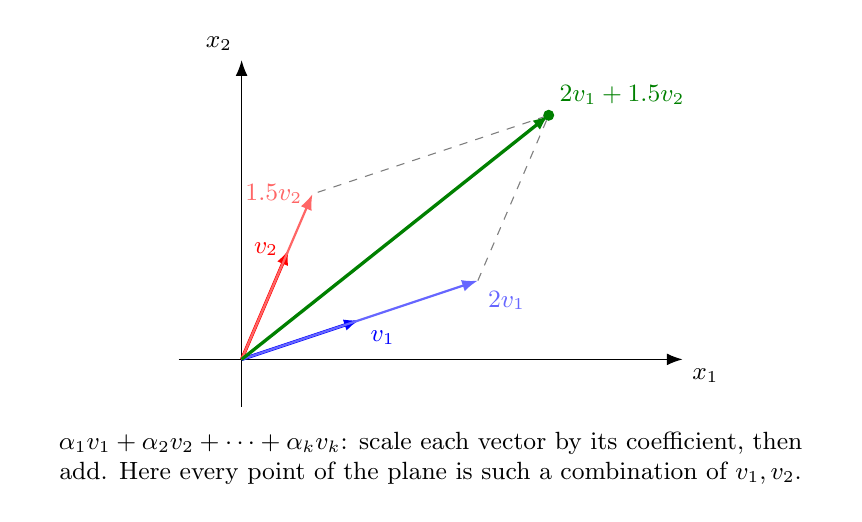
\begin{tikzpicture}[every node/.style={font=\small}, >={Latex[length=2mm]}]
	\draw[->] (-0.8,0) -- (5.6,0) node[below right] {$x_1$};
	\draw[->] (0,-0.6) -- (0,3.8) node[above left] {$x_2$};
	\draw[->, blue, very thick] (0,0) -- (1.5,0.5) node[below right] {$v_1$};
	\draw[->, red, very thick] (0,0) -- (0.6,1.4) node[left] {$v_2$};
	\draw[->, blue!60, thick] (0,0) -- (3,1) node[below right, font=\small] {$2v_1$};
	\draw[->, red!60, thick] (0,0) -- (0.9,2.1) node[left] {$1.5v_2$};
	\draw[dashed, gray] (3,1) -- (3.9,3.1) -- (0.9,2.1);
	\draw[->, green!50!black, very thick] (0,0) -- (3.9,3.1) node[above right] {$2v_1+1.5v_2$};
	\fill[green!50!black] (3.9,3.1) circle (2pt);
	\node[anchor=north, align=flush center, text width=10cm] at (2.4,-0.8) {$\alpha_1v_1+\alpha_2v_2+\cdots+\alpha_kv_k$: scale each vector by its coefficient, then add. Here every point of the plane is such a combination of $v_1,v_2$.};
\end{tikzpicture}
\end{document}
